\documentclass[hyperref={unicode}, xcolor=dvipsnames, t]{beamer}

\usepackage[english]{babel}
\usepackage[utf8]{inputenc}
\usepackage[T1]{fontenc}
\usepackage{csquotes}
\usepackage{biblatex}
\usepackage{graphicx}
\usepackage{animate}

\addbibresource{literature.bib}
\usepackage{booktabs}
\usetheme[
  workplace=fi,
]{MU}
\usepackage{calculator}
\usepackage[acronym]{glossaries}
\makeglossaries
\loadglsentries{acronyms}

\title[Single Image Super-Resolution]{Single Image Super-Resolution}

\author[Mikuláš Bankovič]{Mikuláš Bankovič}
\institute[FI MU]{Faculty of Informatics, Masaryk University}
\date{\today}
\subject{Single Image Super-Resolution: SRCNN and ESPCN}
\keywords{computer vision, machine learning, super-resolution}


\begin{document}

\begin{frame}[plain]
\maketitle
\end{frame}

\section[Introduction]{Introduction}

\begin{frame}{Introduction}{Motivation}
    Why \gls{sr}? \href{https://www.youtube.com/watch?v=Vxq9yj2pVWk}{\structure{Link}} 
    
    \begin{itemize}
      \item<2-8> Games
      \item<3-8> \alert{Medical imaging}
      \item<4-8> Photography details
      \item<5-8> Astronomy
      \item<6-8> \alert{Face and character recognition}
      \item<7-8> \alert{Project \structure{video699}\cite{video699}}
      \item<8-8> Super-scaling of \alert{FFFI} movies
    \end{itemize}
    
    \begin{center}
        \only<2>{
            \vspace{-3cm}
            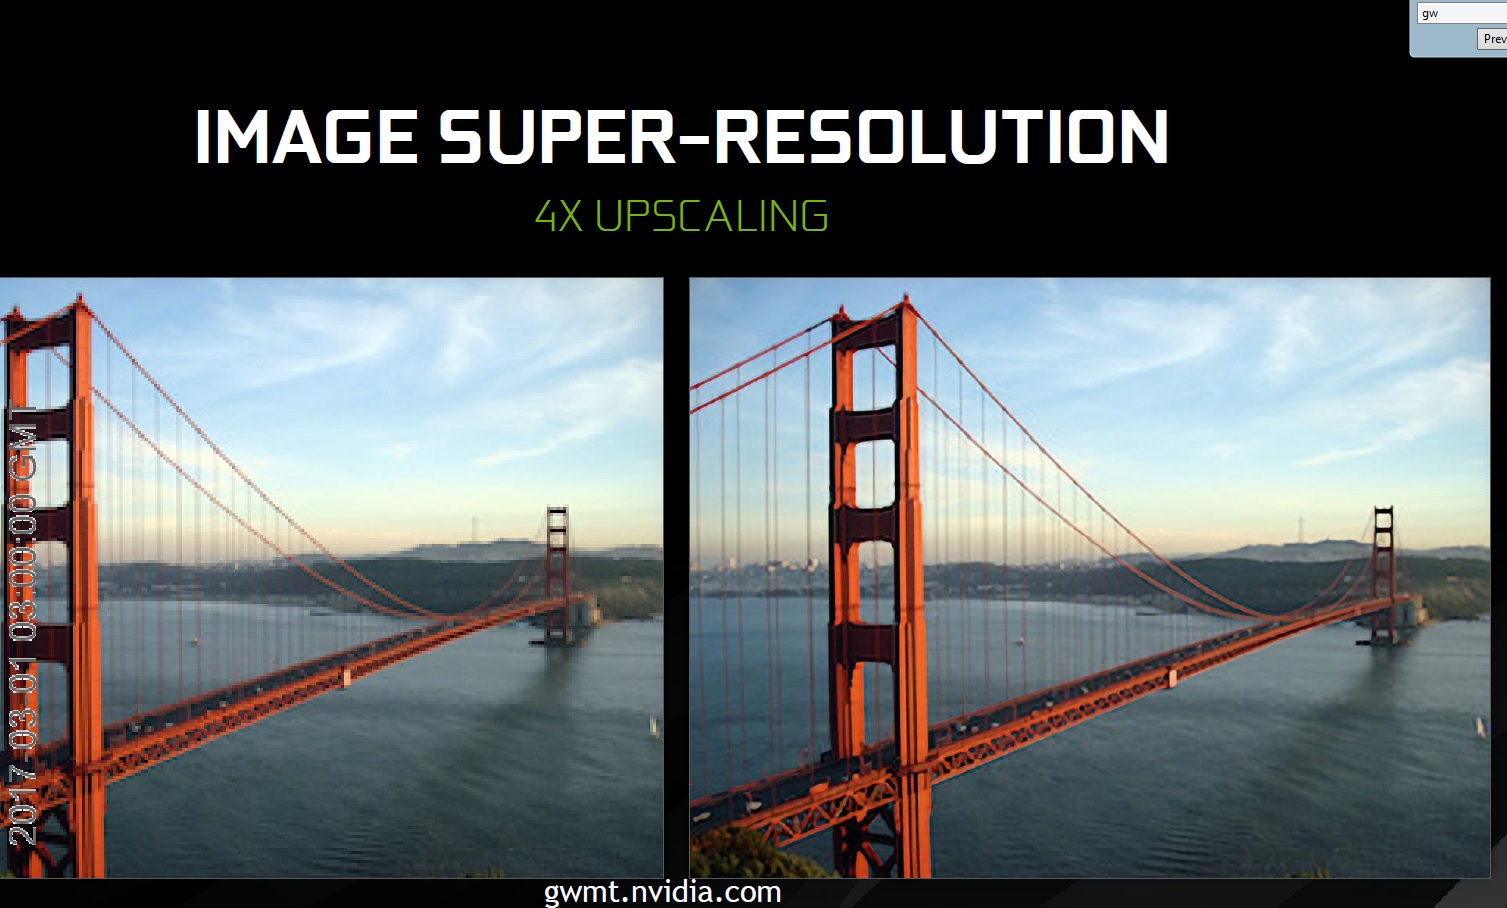
\includegraphics[height=0.5\textheight]{figures/games.png}
        }
        \only<3>{
            \vspace{-3cm}
            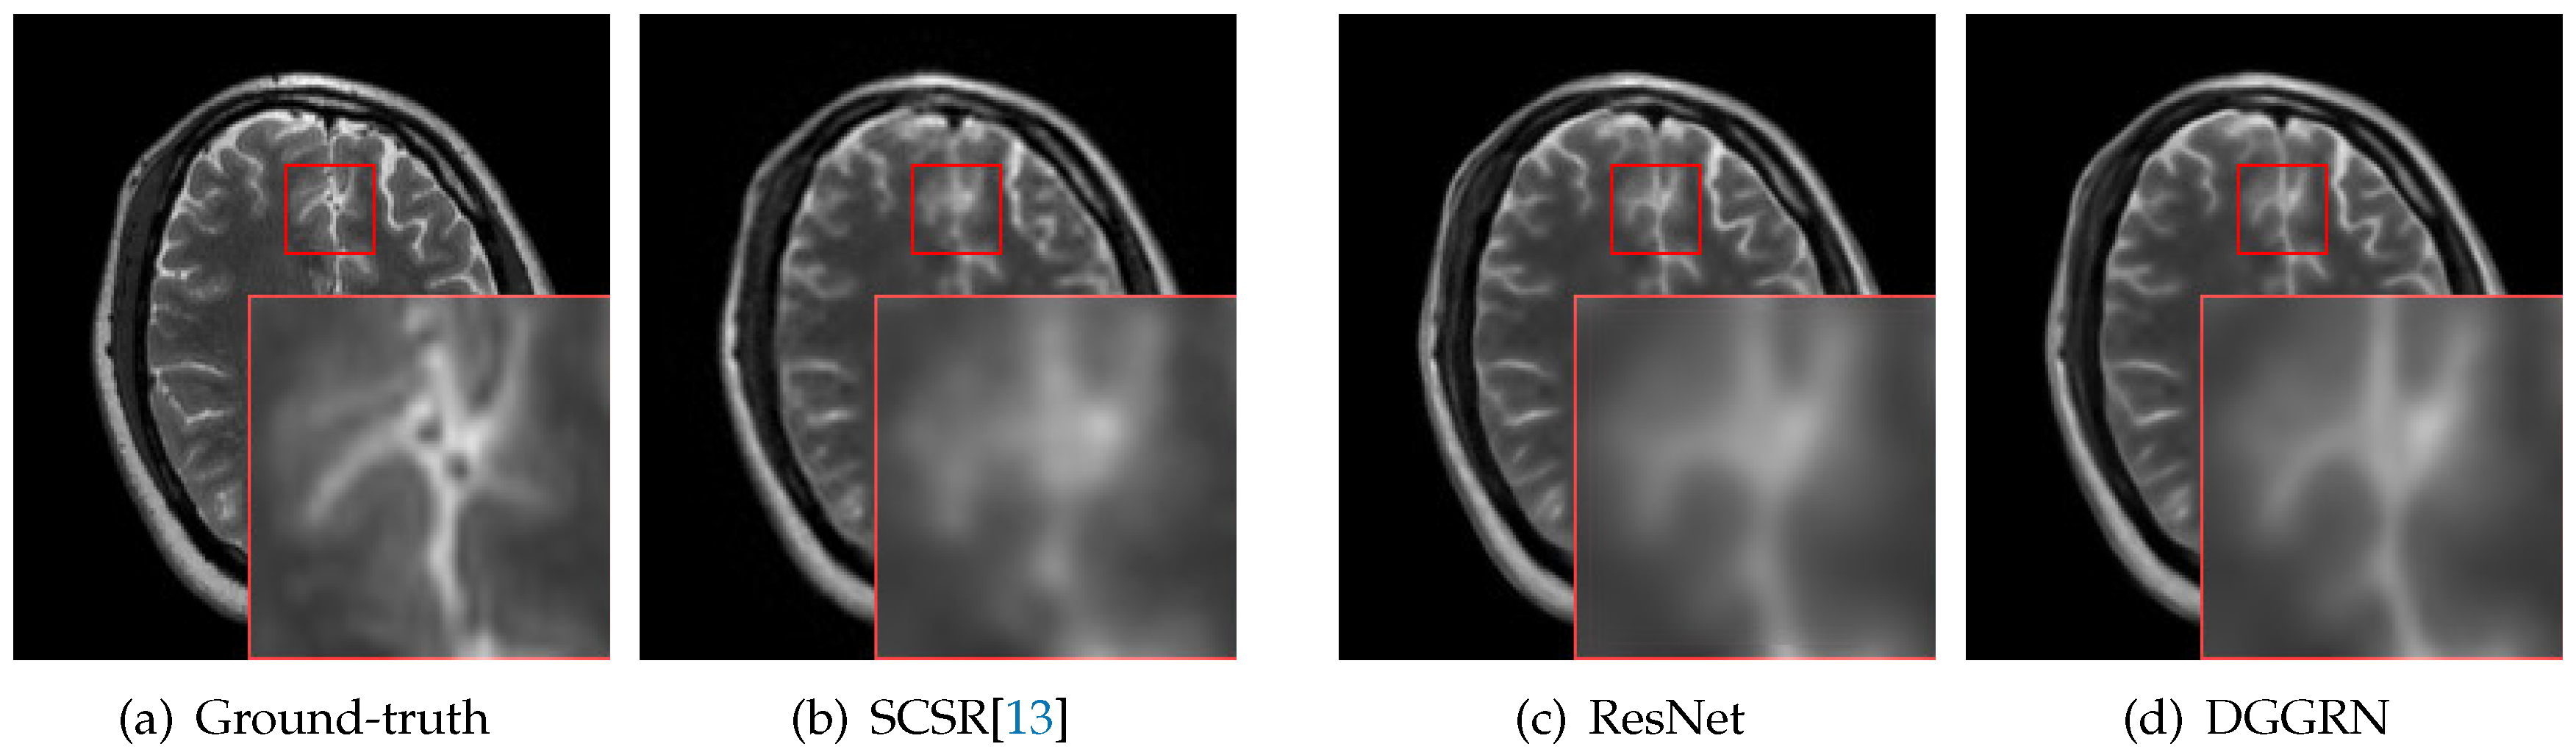
\includegraphics[height=0.4\textheight]{figures/medical.png}
        }
        \only<4>{
        \vspace{-2cm}
            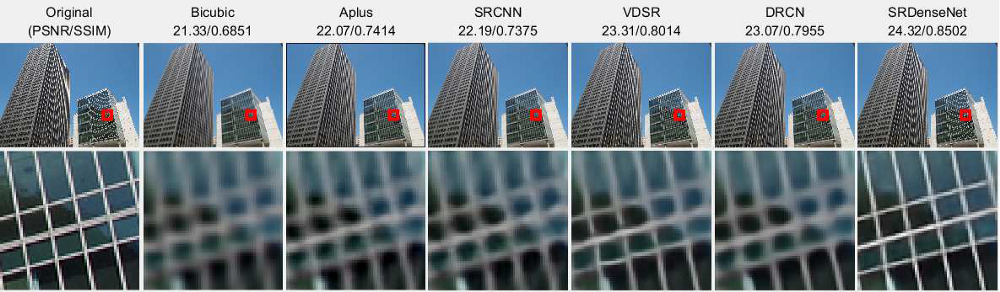
\includegraphics[height=0.4\textheight]{figures/building.png}
        }
        \only<5>{
        \vspace{-2cm}
            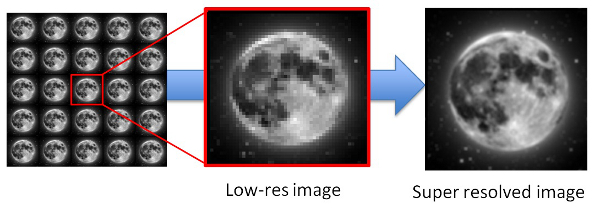
\includegraphics[height=0.4\textheight]{figures/astronomy.jpeg}
        }
    \end{center}
\end{frame}

\begin{frame}{Metrics}
    \begin{itemize}
        \item<1-3> The \gls{psnr} (in dB) is defined as following:
        $$ PSNR =  10\times\log_{10} \left(\frac{MAX^2_I}{MSE}\right), $$
        where $MAX_I$ is the maximum possible pixel value of the image. When the pixels are represented using 8 bits per sample, this is 255. 
        \item<2-3> \gls{ssim} - weighted combination of luminance, contrast and structure:
        \only<2>{
            $$ 
            l(x,y)=\frac{2\mu_x\mu_y + c_1}{\mu^2_x + \mu^2_y + c_1},        c(x,y)=\frac{2\sigma_x\sigma_y + c_2}{\sigma_x^2 + \sigma_y^2 + c_2} $$
            $$ s(x,y)=\frac{\sigma_{xy} + c_3}{\sigma_x \sigma_y + c_3},  c_3 = c_2 / 2 $$
            $$ \text{SSIM}(x,y) = \left[ l(x,y)^\alpha \cdot c(x,y)^\beta \cdot s(x,y)^\gamma \right] $$
        }
        
        \item<3> \gls{mos} - mostly human opinions on 5 number scale
    \end{itemize}
\end{frame}

\begin{frame}{History of \gls{sr}}
Bilinear and \alert{bicubic} interpolation:
\begin{itemize}
    \item no \alert{prior knowledge} about images
    \item no way to \alert{fine-tune to specific dataset}
    \item does not improve with \alert{more data}
\end{itemize}

Sparse-coding-based methods:
\begin{itemize}
    \item The methods are part of example-based learning methods.
    \item They consist of a \alert{multiple-step pipeline}:
    \begin{enumerate}
        \item Crop overlapping patches and preprocess them (substract mean and normalize)
        \item Encode these patches by \gls{lr} dictionary
        \item Encoded coefficients are passed to the \gls{hr} dictionary
        \item Overlapping \gls{hr} patches are aggregated
    \end{enumerate}
    \item Focus on optimizing and improving dictionaries with mapping, while \alert{disregarding other steps}.
    \item They often have to solve \alert{optimization problems on inference}.
\end{itemize}
\end{frame}

\section{SRCNN}
\begin{frame}{\texorpdfstring{\gls{srcnn}}{Lg}}
    \begin{itemize}
        \item Given by \textcite{srcnn}, the \gls{cnn} is \alert{equivalent} to the previous pipeline.
        \item That brings multiple advantages:
        \begin{itemize}
            \item The inference consists only from \alert{feed-forward pass}.
            \item The pipeline is unified, therefore, each step is optimized during training.
            \item The dictionaries are not explicitly formed, but included in the weights.
            \item Provides \alert{superior quality and speed performance} (Next slides).
        \end{itemize}
    \end{itemize}
\end{frame}

\begin{frame}{\texorpdfstring{\gls{srcnn}}{Lg}}
    \begin{itemize}
        \item<1> \gls{srcnn} is a simple \gls{cnn} with \alert{three} convolutional layers.
        \item<1> The input image is firstly upscaled using bicubic interpolation.
        \item<1> The next step is feed-forward pass through the network.
        \item<1> The different architecture involved changes in filter size: 9-1-5, 9-5-5, 11-5-7, etc.
    \end{itemize}
    
    \begin{center}
        \only<2>{
            \vspace{-2.5cm}
            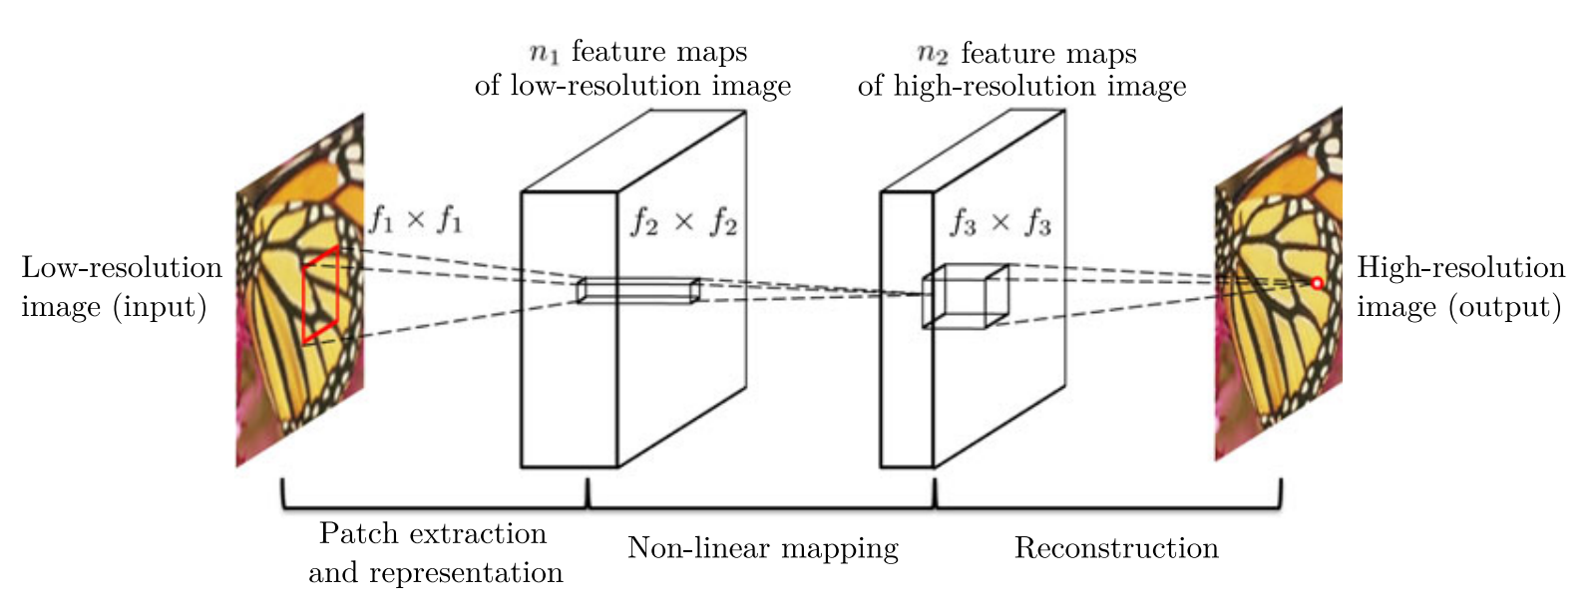
\includegraphics[height=\textheight,width=\textwidth,keepaspectratio]{figures/srcnn.png}
        }
        \only<3>{
            \vspace{-3cm}
            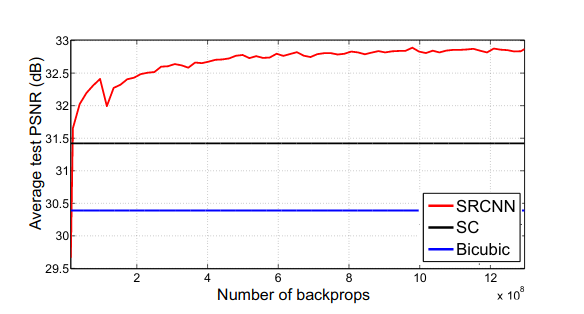
\includegraphics[height=\textheight,width=\textwidth,keepaspectratio]{figures/performance.png}
        }
        \only<4>{
        \vspace{-3cm}
            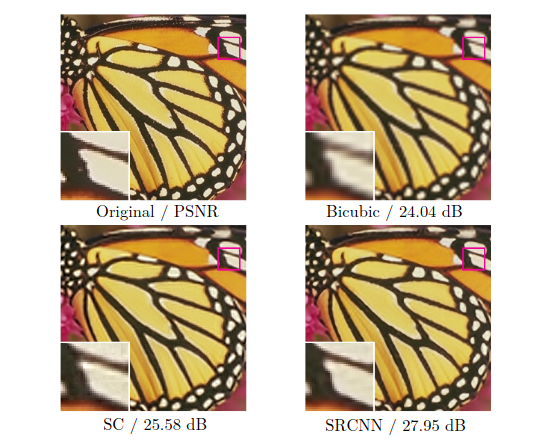
\includegraphics[height=0.9\textheight,width=0.9\textwidth,keepaspectratio]{figures/example.png}
        }
        \only<5>{
        \vspace{-2.5cm}
            
\includegraphics[height=0.9\textheight,width=0.9\textwidth,keepaspectratio]{figures/waifu.png}
        }
        % \only<6>{
        % \vspace{-2.5cm}
        %     \includegraphics[height=\textheight, width=\textwidth, keepaspectratio]{figures/waifu2.png}
        % }
    \end{center}
\end{frame}

\begin{frame}{Problems}
    \begin{itemize}
        \item The \alert{bicubic interpolation} is an expensive operation that often introduce side-effects as blurring or noise amplification.
        \item More data could \alert{overfit} the network, because its smaller size.
        \item Most of the operations are performed in an expensive \alert{\gls{hr}} space.
    \end{itemize}
\end{frame}

\section{FSRCNN}
\begin{frame}{\texorpdfstring{\gls{fsrcnn}}{Lg}}
    The main differences between \gls{srcnn} and \gls{fsrcnn}:
    \begin{itemize}
        \item There is no pre-processing or upsampling at the beginning. The feature extraction took place in the \alert{\gls{lr} space}.
        \item A $1\times1$ convolution is used after the initial $5\times5$ convolution to reduce the number of channels, and hence lesser computation and memory, similar to how the Inception\cite{inception} network is developed.
        \item Multiple $3\times3$ convolutions are used, instead of having a big convolutional filter, similar to how the VGG network works by simplifying the architecture to reduce the number of parameters.
        \item Upsampling is done by using a learnt transposed convolution, thus improving the model.
    \end{itemize}
\end{frame}

\begin{frame}{\texorpdfstring{\gls{fsrcnn}}{Lg}}
     \begin{itemize}
        \item 17.36 times faster than \gls{srcnn} and can run in real time (24 fps) with a generic CPU.
        \item All layers except from the last can be shared with multiple upscaling factors.
        \item Transposed convolution \href{https://i.stack.imgur.com/YyCu2.gif}{\structure{LINK}}\cite{conv_operations}
        \item Transposed convolution with stride \href{https://i.stack.imgur.com/f2RiP.gif}{\structure{LINK}}\cite{conv_operations}
    \end{itemize}
\end{frame}

\begin{frame}{\texorpdfstring{\gls{fsrcnn}}{Lg}}
    \begin{center}
        \only<1>{
            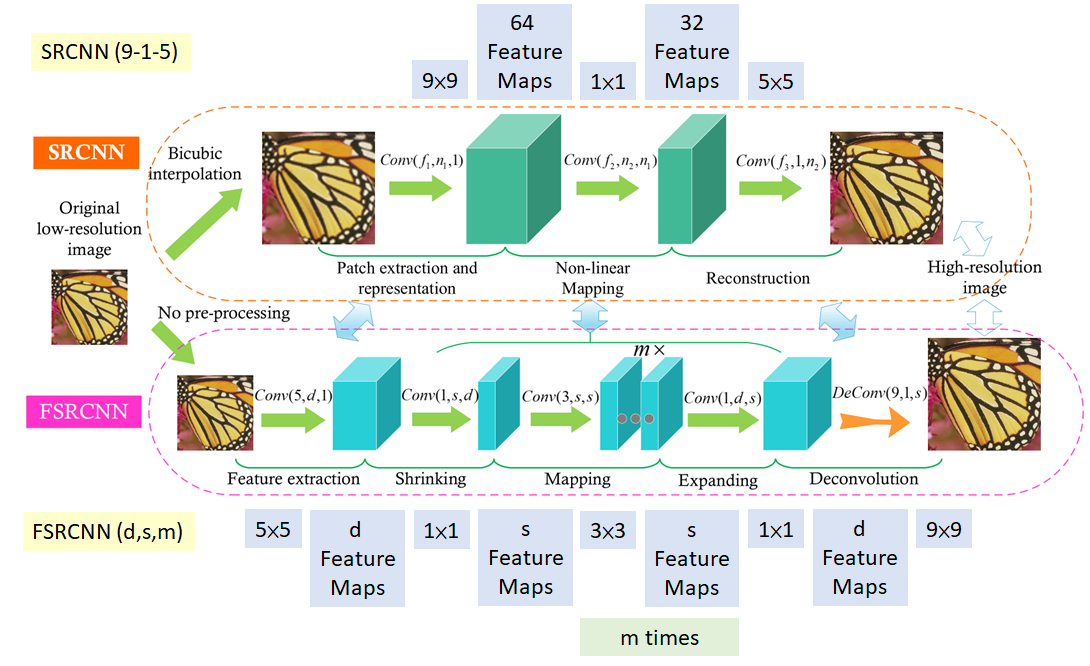
\includegraphics[width=0.9\linewidth, height=0.9\textheight,keepaspectratio]{figures/fsrcnn.png}
        }
        \only<2>{
            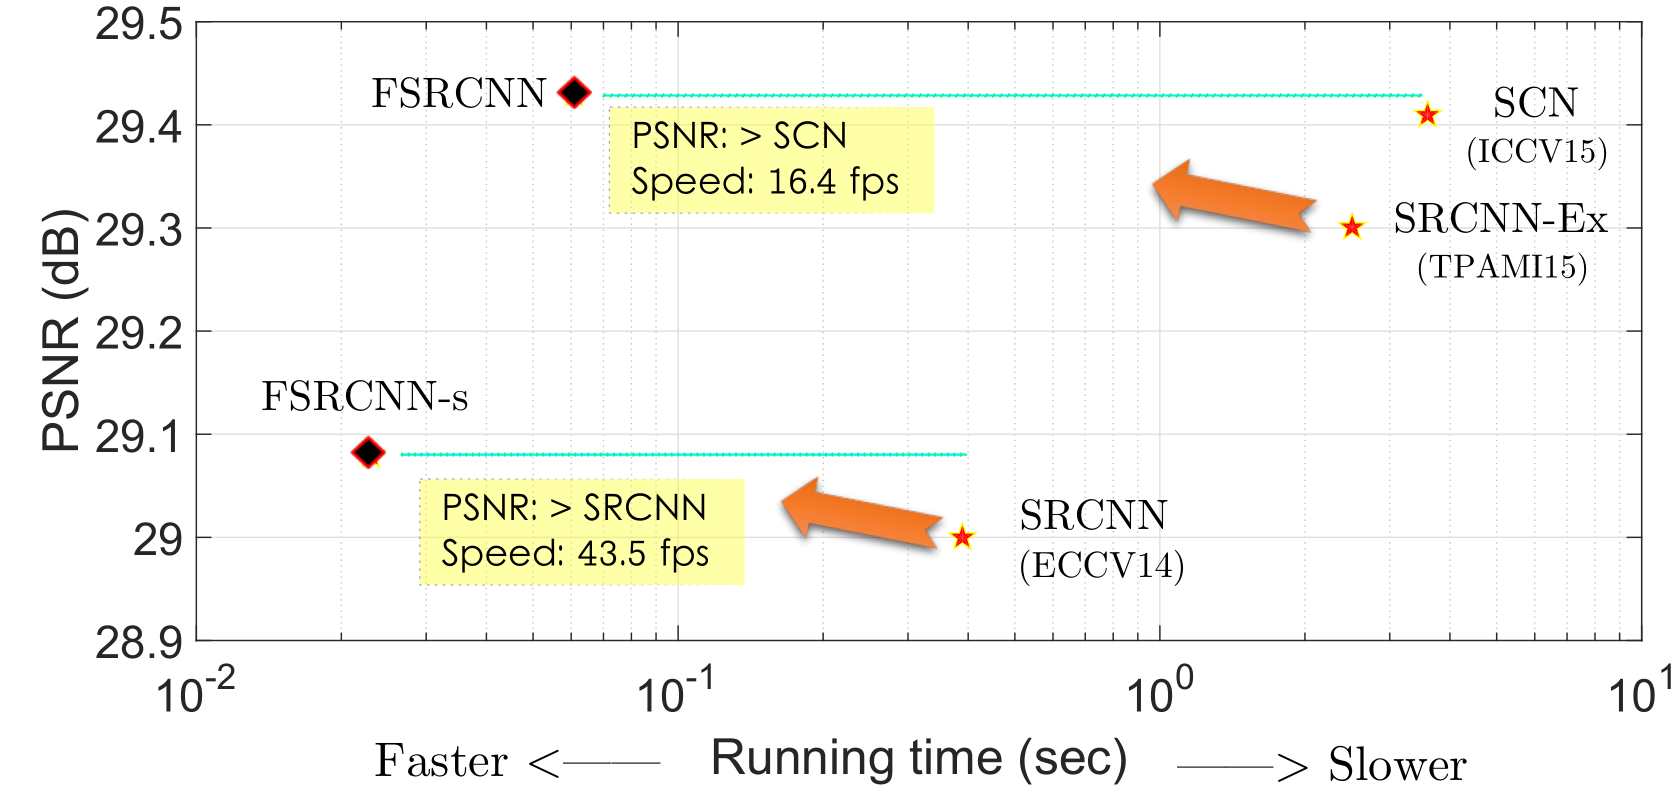
\includegraphics[width=0.9\linewidth, height=0.9\textheight,keepaspectratio]{figures/fsrcnn1.png}
        }
        \only<3>{
            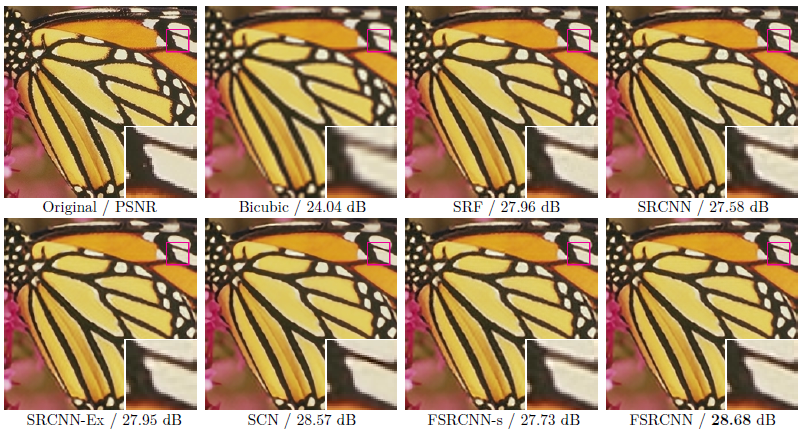
\includegraphics[width=0.9\linewidth, height=0.9\textheight,keepaspectratio]{figures/fsrcnn-example.png}
        }
    \end{center}
\end{frame}

\section{ESPCN}
\begin{frame}{\texorpdfstring{\gls{espcn}}{Lg}}
    \begin{itemize}
        \item \gls{espcn} introduces the concept of sub-pixel convolution to replace the transposed convolution layer for upsampling. This solves two problems associated with it:
        \begin{enumerate}
            \item Transposed convolution happens in the high resolution space, and thus is more computationally expensive.
            \item It resolves the checkerboard issue in deconvolution, which occurs due to the overlap operation of convolution.
        \end{enumerate}
    \end{itemize}
    \begin{center}
        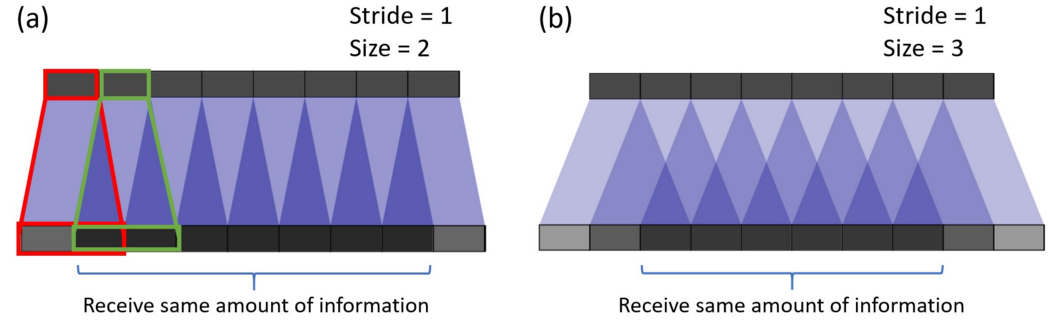
\includegraphics[keepaspectratio, height=0.4\textheight]{figures/trans_conv_problem.png}
    \end{center}
\end{frame}

\begin{frame}{Sub-pixel convolutional layers}
    \begin{itemize}
        \item In the more up-to-date literature they are called pixel-shuffle layers.
        \item Sub-pixel convolution works by converting depth to space, as seen in the figure below. 
        \item Pixels from multiple channels in a low resolution image are rearranged to a single channel in a high resolution image. 
    \end{itemize}
    \begin{center}
    \only<1> {
        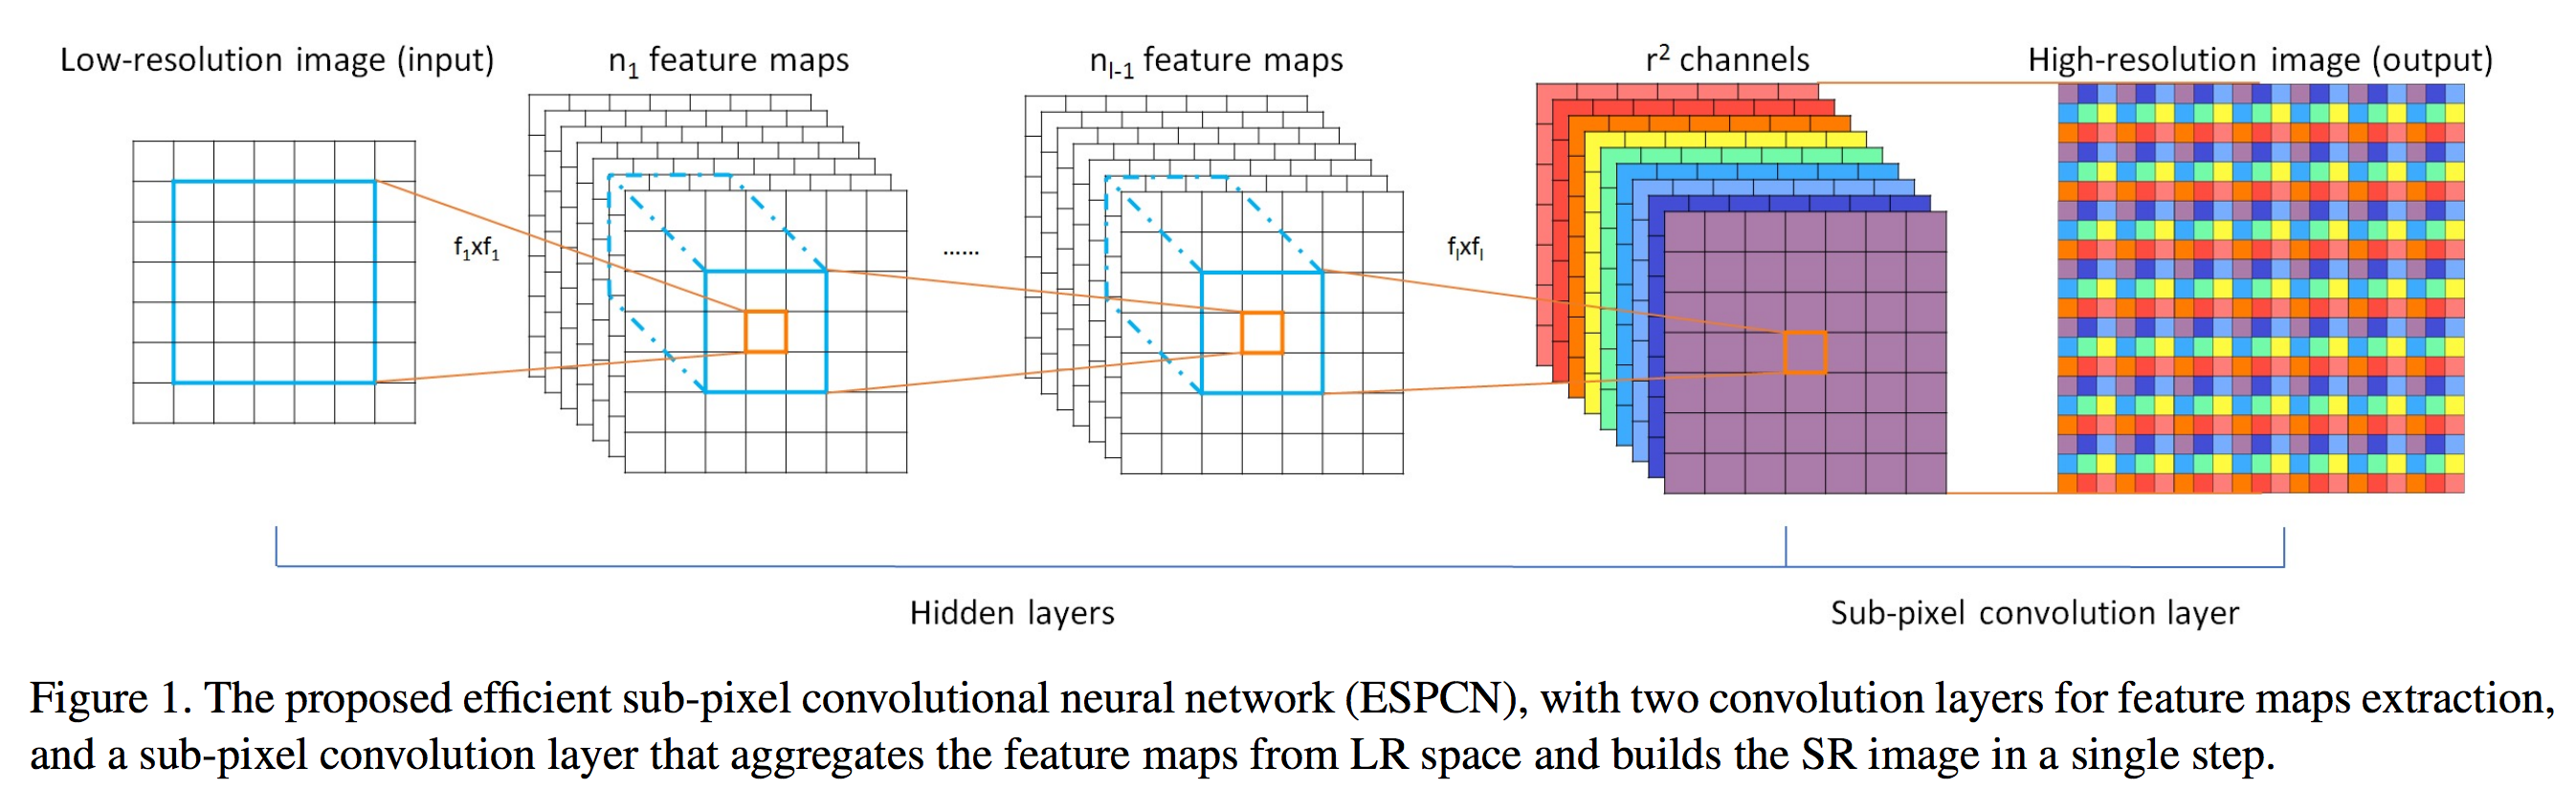
\includegraphics[width=\linewidth]{figures/sub-pixel.png}
    }
    \only<2> {
        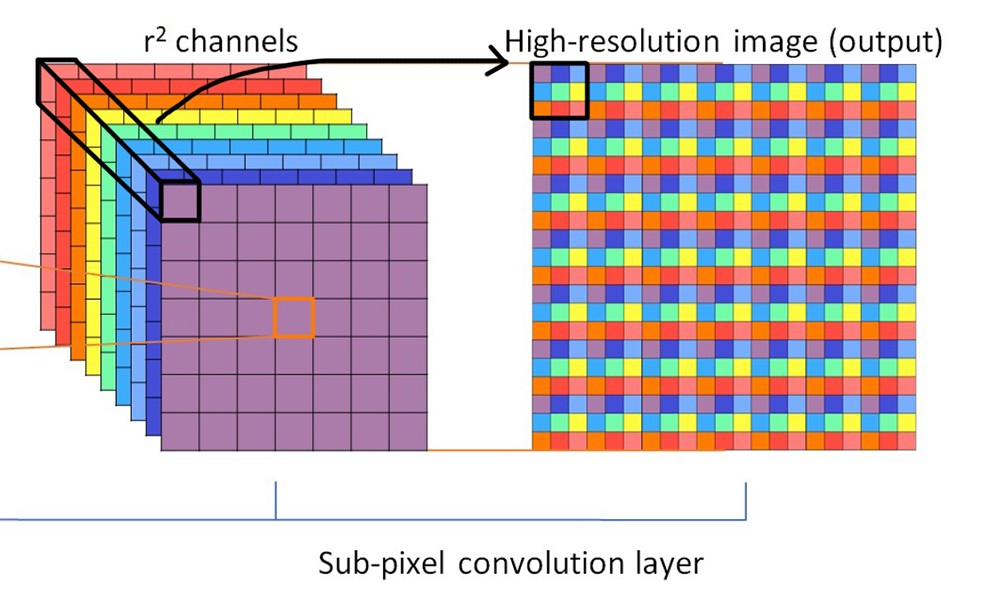
\includegraphics[width=0.8\linewidth]{figures/sub-pixel-detail.jpeg}
    }
    \end{center}
\end{frame}

\begin{frame}{\texorpdfstring{\gls{espcn}}{Lg}}
    \begin{center}
        \includegraphics[height=\textheight,width=\textwidth,keepaspectratio]{figures/}
    \end{center}    
\end{frame}

\section{SRGAN}
\begin{frame}{\texorpdfstring{\gls{srgan}}{Lg}}
    \begin{itemize}
        \item<1,3> Problem: All previous methods were train on MSE loss function. However, ideal MSE image is not offhand the most photo-realistic
        \item<1,3> Solution: \gls{gan}
        \newline
        \item<3> Problem: As in other computer vision disciplines, deeper models are more successful, however, harder to train due to some aspects, such as vanishing gradient problem.
        \item<3> Solution: ResNet
    \end{itemize}
    
    \begin{center}
        \only<2>{
            \vspace{-5.5cm}
            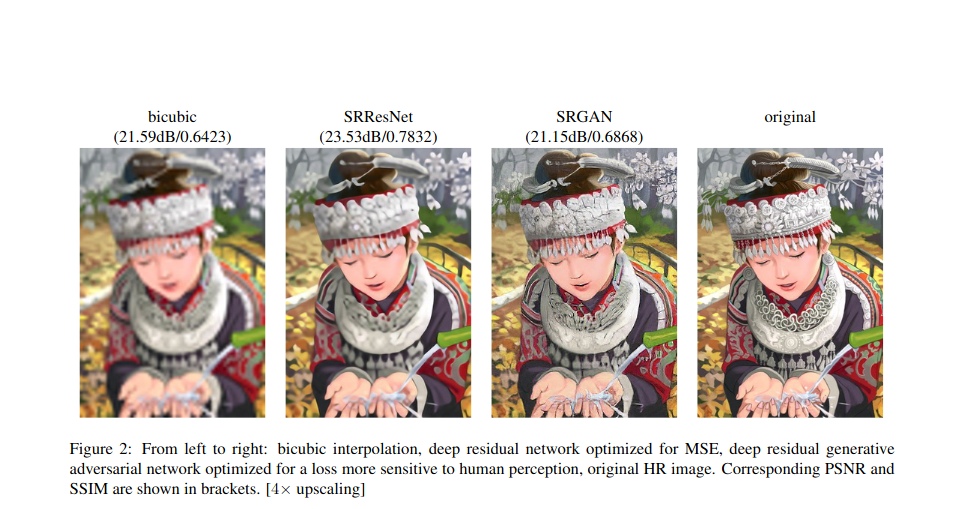
\includegraphics[keepaspectratio,width=1.1\textwidth,height=1.1\textheight]{figures/psnr_metric.png}   
        }
    \end{center}
    
\end{frame}


\begin{frame}{ResNet}
    \begin{center}
        \only<1>{
            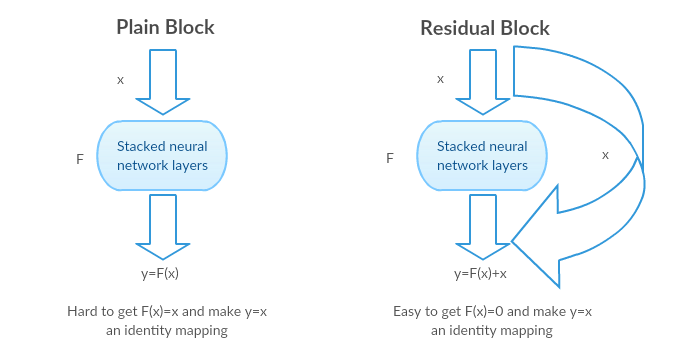
\includegraphics[keepaspectratio,width=\linewidth]{figures/residual_connections.png}
        }
    \end{center}
\end{frame}

\begin{frame}{GAN}
    \only<1>{
            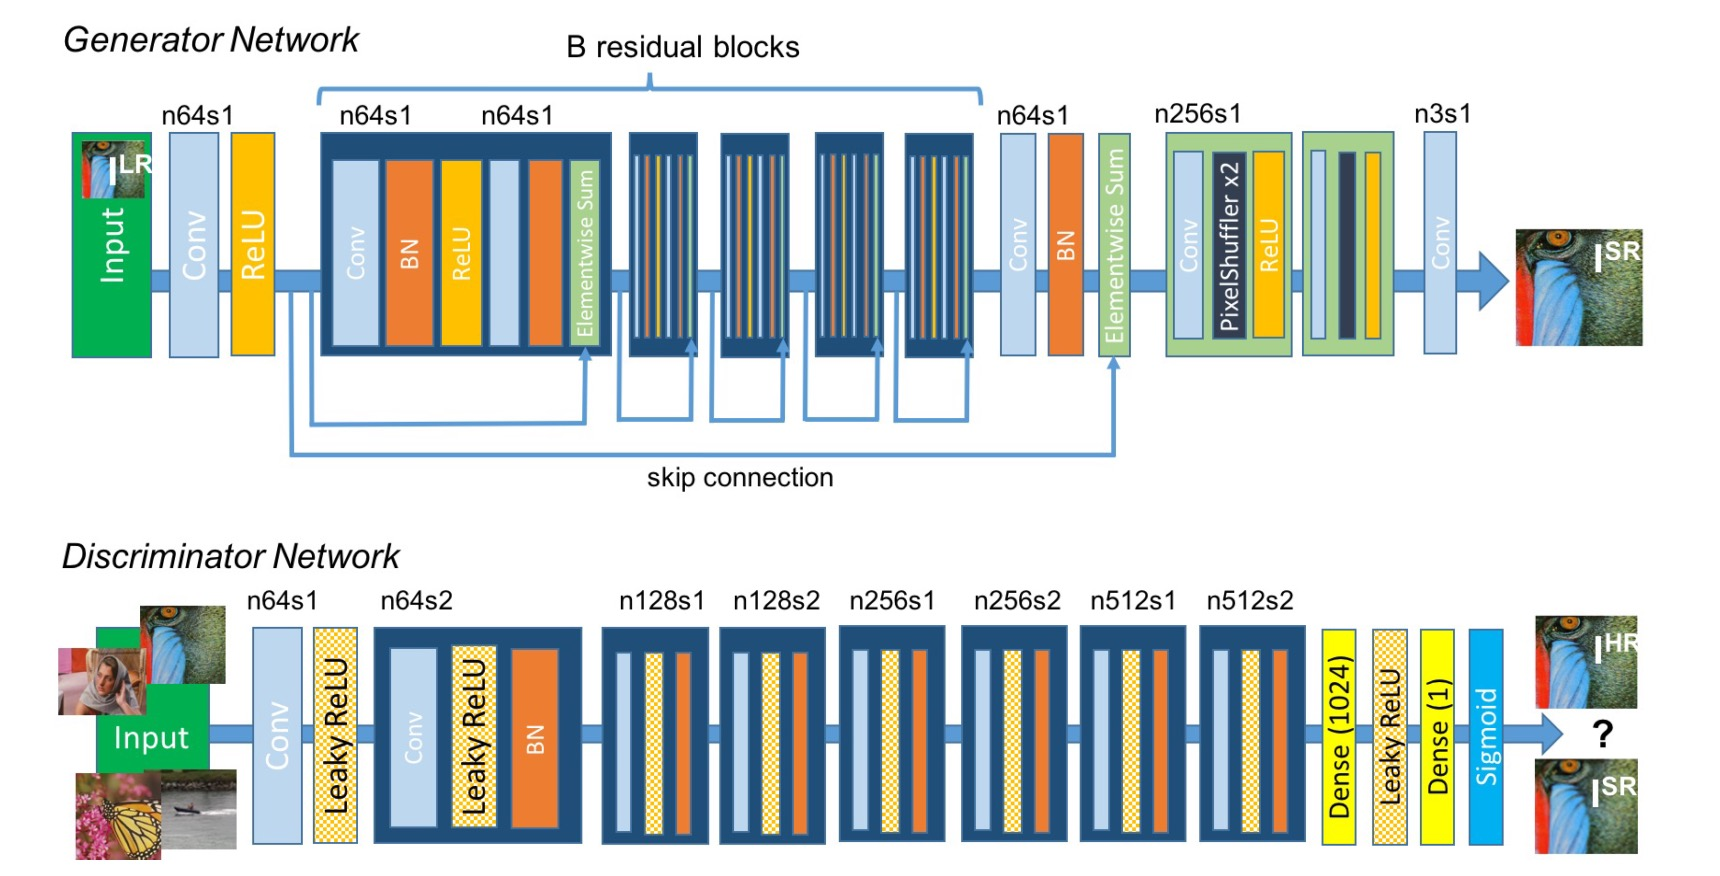
\includegraphics[keepaspectratio,width=\linewidth]{figures/srgan.jpeg}
    }
\end{frame}

\begin{frame}{SRGAN}
    \begin{itemize}
        \item This paper generates \gls{sota} results on upsampling (4x) as measured by \gls{psnr} and \gls{ssim} with 16 block deep SRResNet network optimized for MSE.
        \item The authors proposed a new \gls{srgan} in which the authors replace the MSE based content loss with the loss calculated on VGG layers.
        \item \gls{srgan} was able to generate \gls{sota} results which the author validated with extensive \gls{mos} test on three public benchmark datasets.
        \item Use 2 losses for generator network: MSE and function based on the euclidean distance  between feature maps extracted from the VGG19 network.
    \end{itemize}
\end{frame}

\begin{frame}{Future}
    \begin{itemize}
        \item Residual networks?
        \item Attention-based networks?
        \item GANs?
        \item Progressive Reconstruction Networks?
    \end{itemize}
\end{frame}

\begin{frame}[plain]
\vfill
\centerline{Thank You for Your Attention!}
\vfill\vfill
\end{frame}

\section{\bibname}
\begin{frame}[t, allowframebreaks]{\bibname}
\printbibliography[heading=none]
\end{frame}



\printglossary[type=\acronymtype]

\end{document}
